% diagrams/english/cometa.tex -- la cometa de Dad, para "Read and
% colour": un rombo partido en cuatro por las dos varillas (dos partes
% arriba y dos abajo), y la cola con cuatro lazos.
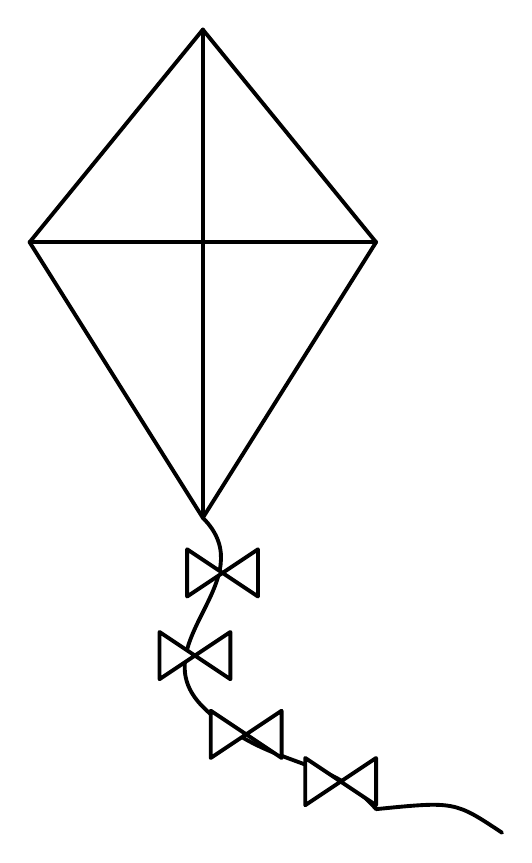
\begin{tikzpicture}[line width=1.4pt, line cap=round, line join=round, scale=1.0]
  % el rombo y las varillas
  \filldraw[fill=white] (0,4.6) -- (2.2,1.9) -- (0,-1.6) -- (-2.2,1.9) -- cycle;
  \draw (0,4.6) -- (0,-1.6); \draw (-2.2,1.9) -- (2.2,1.9);
  % la cola
  \draw (0,-1.6) .. controls (0.8,-2.4) and (-0.8,-3.2) .. (0,-4.0)
                 .. controls (0.8,-4.8) and (1.6,-4.6) .. (2.2,-5.3);
  % los cuatro lazos
  \foreach \x/\y in {0.25/-2.3, -0.1/-3.35, 0.55/-4.35, 1.75/-4.95} {
    \filldraw[fill=white] (\x,\y) -- ++(-0.45,0.3) -- ++(0,-0.6) -- cycle;
    \filldraw[fill=white] (\x,\y) -- ++(0.45,0.3) -- ++(0,-0.6) -- cycle;
  }
  % el hilo
  \draw (2.2,-5.3) .. controls (3.2,-5.2) .. (3.8,-5.6);
\end{tikzpicture}
